\section*{mapping SoRa}

\lipsum{1-9}
\begin{figure}[H]
    \centering
    \ifodd\value{page} % Check if the page is odd
        \begin{adjustwidth}{0pt}{0.0\paperwidth} % Adjust right margin for odd pages
            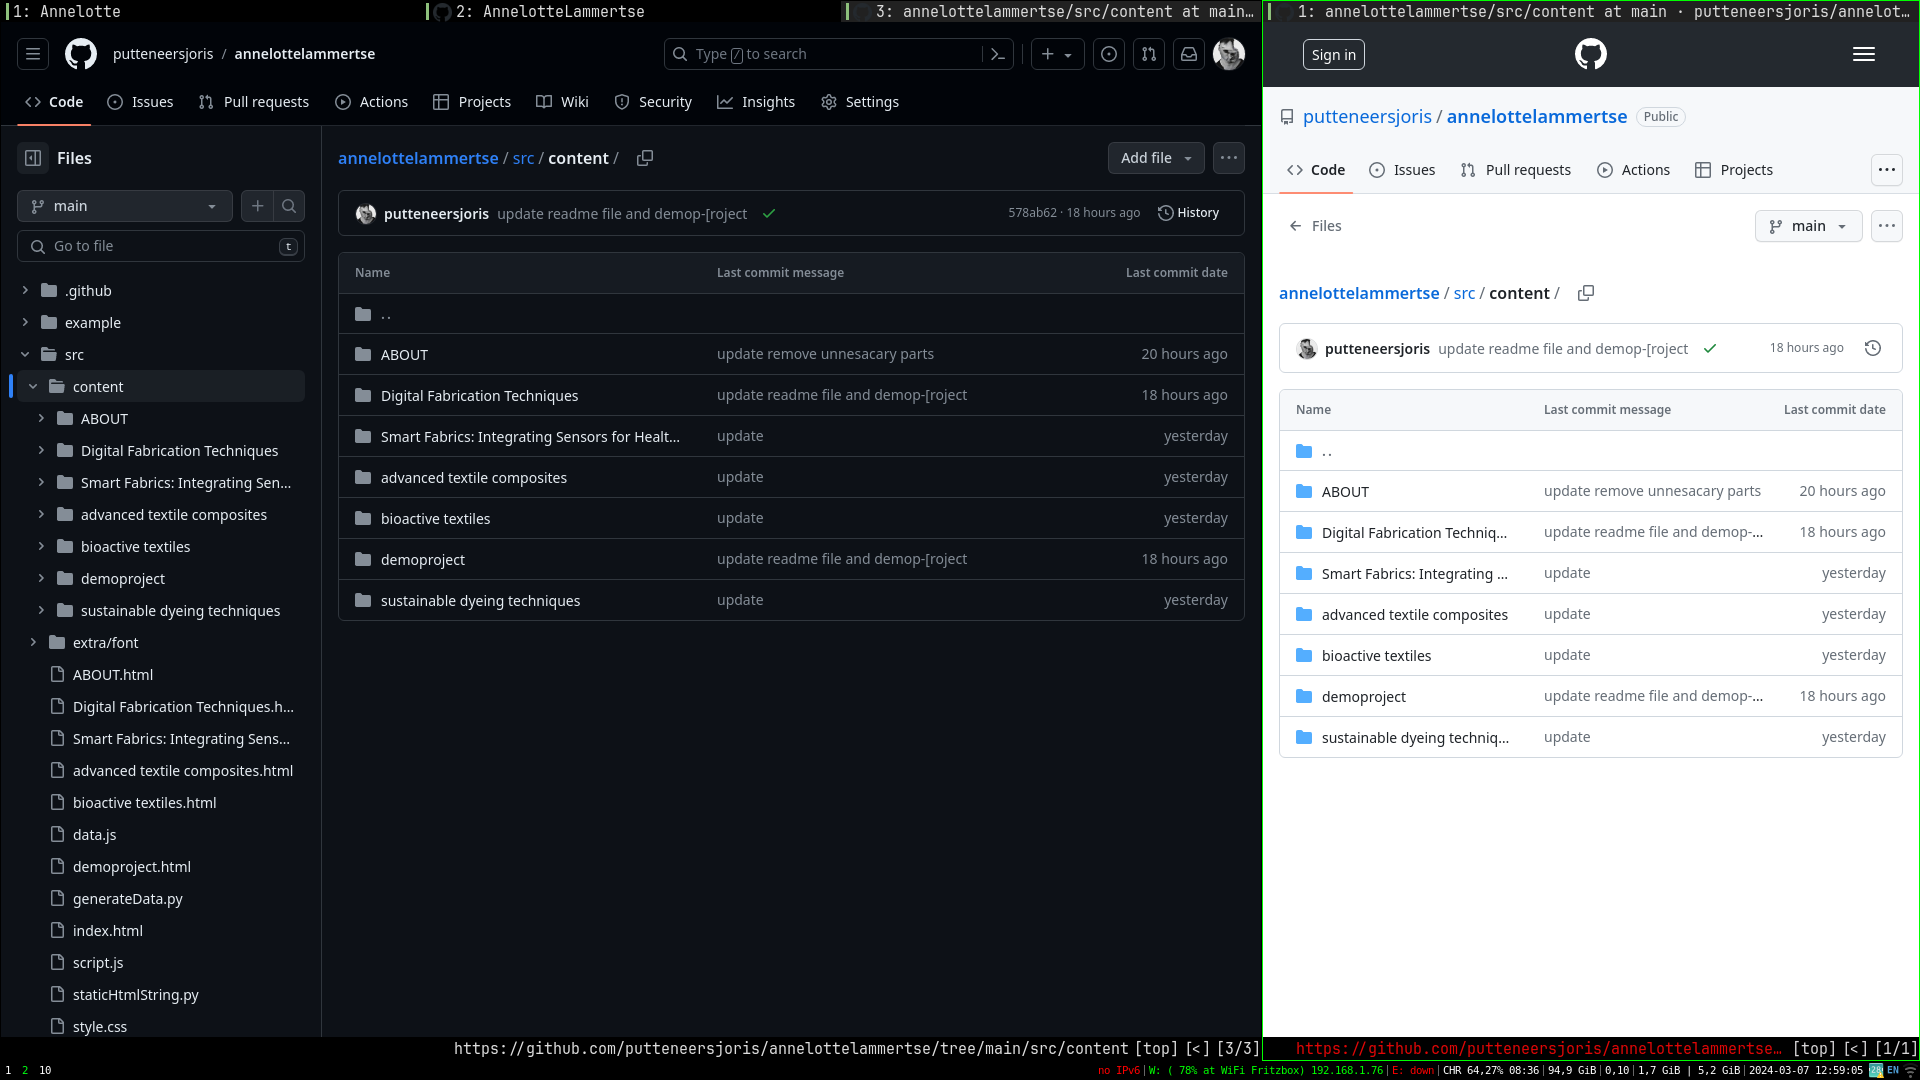
\includegraphics[width=0.9\paperwidth]{sections/assignment_1/1.png}
        \end{adjustwidth}
    \else
        \begin{adjustwidth}{-0.0\paperwidth}{0pt} % Adjust left margin for even pages
            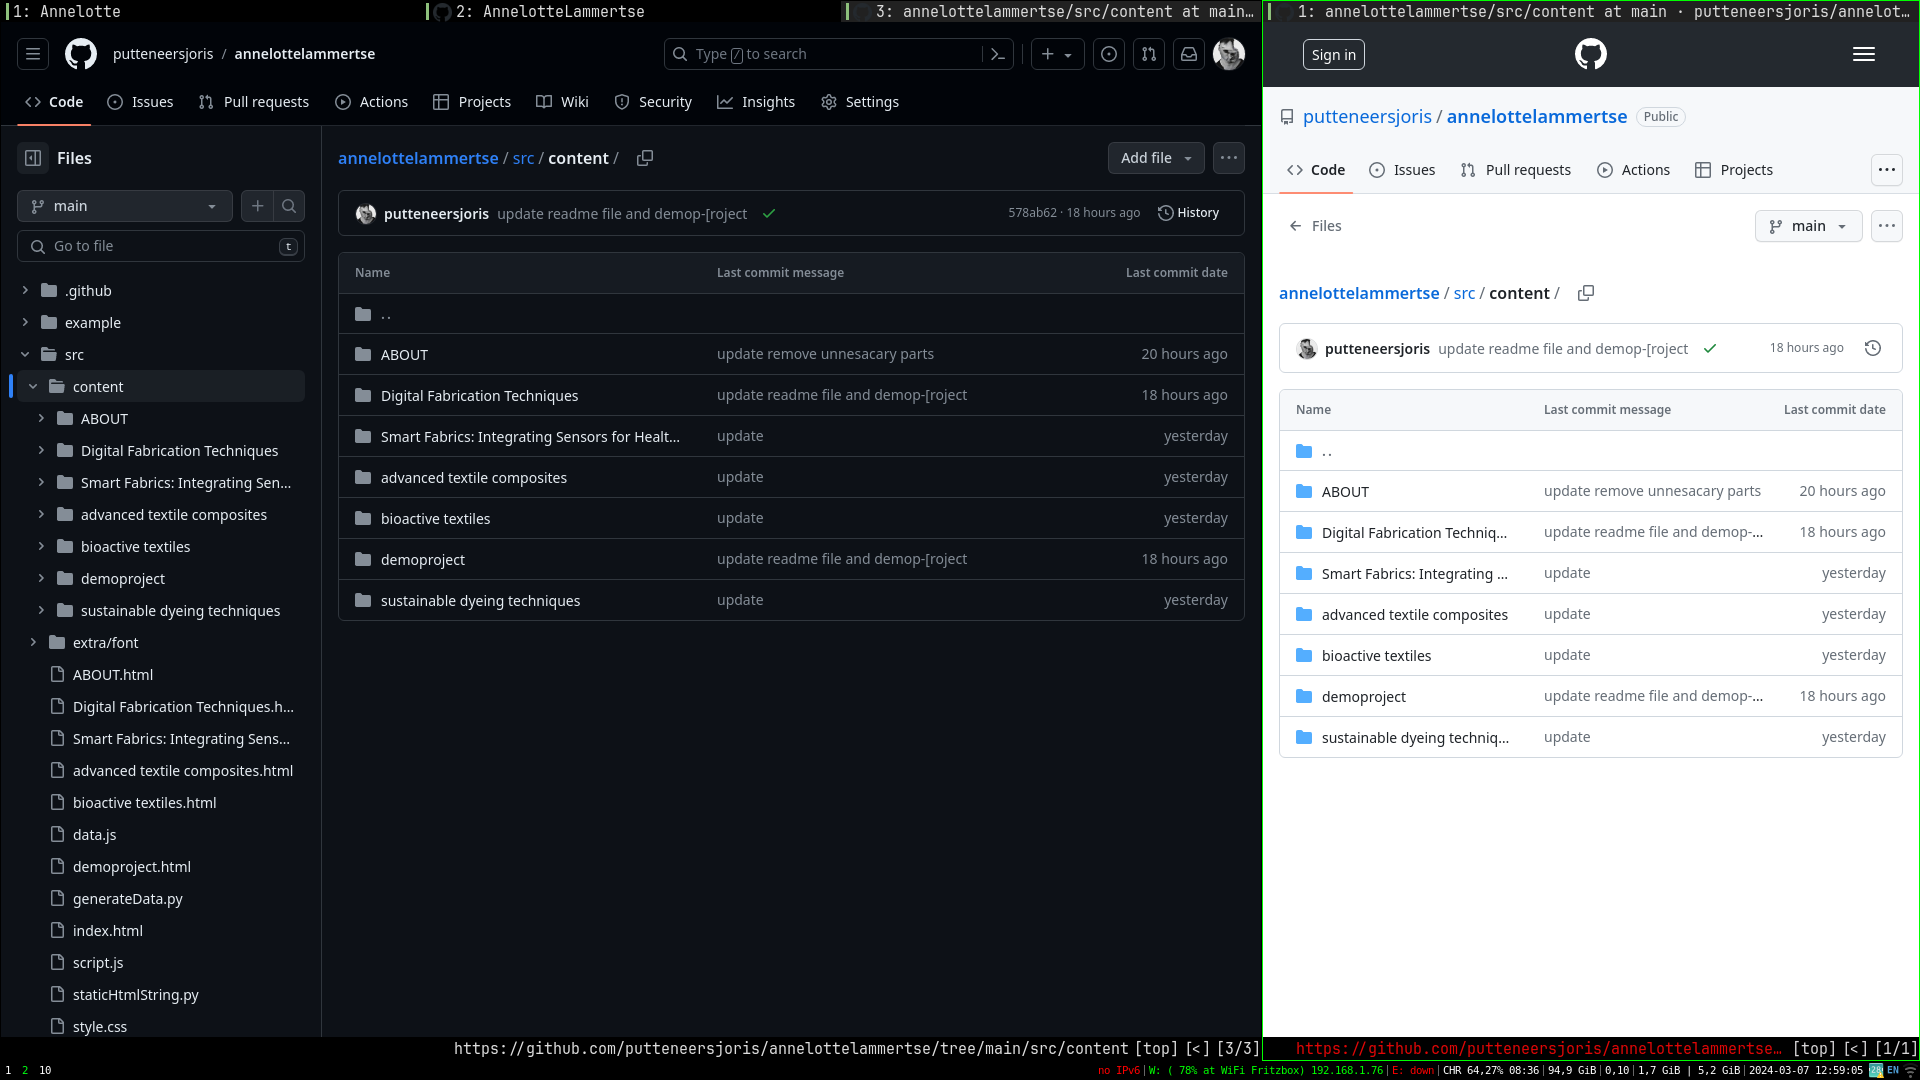
\includegraphics[width=0.9\paperwidth]{sections/assignment_1/1.png}
        \end{adjustwidth}
    \fi
    \caption{A full-page image}
\end{figure}

\lipsum{1-9}

\markboth{\hspace{1cm}exercices}{Joris Putteneers\hspace{1cm}}



word\footnote{Explanation of the word.} that Addjword\footnote{Explanation of the word.} thatjord\footnote{Explanation of the word.} thatYou can find the source code on GitHub: \url{https://github.com/your-username/your-repository}.


\keywords{nnode / context / parameter / attribute / primitive /mitive mitive mitive mitive mitive  vertex / point / object / procedural / datatypenode / context / parameter / attribute / primitive /mitive mitive mitive mitive mitive  vertex / point / object / procedural / datatyp eode / context / parameter / attribute / primitive /mitive mitive mitive mitive mitive  vertex / point / object / procedural / datatype}


